% Permission is granted to copy, distribute and/or modify this document
% under the terms of the GNU Free Documentation License, Version 1.3
% or any later version published by the Free Software Foundation;
% with no Invariant Sections, no Front-Cover Texts, and no Back-Cover Texts.
% A copy of the license is included in the section entitled "GNU
% Free Documentation License".
%
% Written (C) 2012 Heiko Strathmann

\chapter{Statistical Testing}
This chapter describes \shogun{}'s framework for statistical hypothesis testing. We begin by giving a brief outline of the problem setting in section \ref{sec:hypothesis_testing_into}. Then, we describe methods for two-sample testing for independence testing.

Methods for two-sample testing currently consist of tests based on the \emph{Maximum Mean Discrepancy}, section \ref{sec:mmd_into}. There are two types of tests available, a quadratic time test, which is described in section \ref{sec:mmd_quadratic}; and a linear time test, which is described in section \ref{sec:mmd_linear}. Both come in various flavours.

Independence testing is currently based in the \emph{Hilbert Schmidt Independence Criterion}, which is described in section \ref{sec:hsic_test} along with a test using it.

\section{Statistical Hypothesis Testing}
\label{sec:hypothesis_testing_into}

To set the context, we here briefly describe statistical hypothesis testing. Informally, one defines a hypothesis on a certain domain and then uses a statistical test to check whether this hypothesis is true. Formally, the goal is to reject a so-called \emph{null-hypothesis} $H_0$, which is the complement of an \emph{alternative-hypothesis} $H_A$. 

To distinguish the hypothesises, a test statistic is computed on sample data. Since sample data is finite, this corresponds to sampling the true distribution of the test statistic. There are two different distributions of the test statistic -- one for each hypothesis. The \emph{null-distribution} corresponds to test statistic samples under the model that $H_0$ holds; the \emph{alternative-distribution} corresponds to test statistic samples under the model that $H_A$ holds.

In practice, one tries to compute the quantile of the test statistic in the null-distribution. In case the test statistic is in a high quantile, i.e.\ it is unlikely that the null-distribution has generated the test statistic -- the null-hypothesis $H_0$ is rejected.

There are two different kinds of errors in hypothesis testing:
\begin{itemize}
\item A \emph{type I error} is made when $H_0: p=q$ is wrongly rejected. That is, the tests says that the samples are from different distributions when they are not.
\item A \emph{type II error} is made when $H_A: p=q$ is wrongly accepted. That is, the tests says that the samples are from same distributions when they are from the same.
\end{itemize}
A so called \emph{consistent} test achieves zero type II error for a fixed type I error.

To decide whether to reject $H_0$, one could set a threshold, say at the 95\% quantile of the null-distribution, and reject $H_0$ when the test statistic lies below that threshold. This means that the chance that the samples were generated under $H_0$ are 5\%. We call this number the test power $\alpha$ (in this case $\alpha=0.05$). It is an upper bound on the probability for a type I error. An alternative way is simply to compute the quantile of the test statistic in the null-distribution, the so-called \emph{p-value}, and to compare the p-value against a desired test power, say $\alpha=0.05$, by hand. The advantage of the second method is that one not only gets a binary answer, but also an upper bound on the type I error.

In order to construct a two-sample test, the null-distribution of the test statistic has to be approximated. One way of doing this for any two-sample test is called \emph{bootstrapping}:
\begin{algorithm}
Inputs are:
\begin{itemize}
 \item $X,Y$, sets of samples from $p,q$ of size $m,n$ respectively
\end{itemize}
Output is:
\begin{itemize}
 \item One sample from null-distribution. Simply repeat for more samples.
\end{itemize}

 \begin{algorithmic}[1]
\STATE{$Z \gets \{X,Y\}$}
\STATE{$\hat{Z}=\{\hat{z}_1,...,\hat{z}_{m+n}\}\gets \text{randperm}(Z)$} \qquad (generate a random ordering)
\STATE{$\hat{X}\gets \{\hat{z}_1,...\hat{z}_m\}$}
\STATE{$\hat{Y}\gets \{\hat{z}_{m+1},...\hat{z}_{m+n}\}$}
\RETURN{Test statistic for $\hat{X},\hat{Y}$}
\end{algorithmic}
\caption{Bootstrapping a null-distribution.}
\label{alg:bootstrapping}
\end{algorithm}

Bootstrapping is a useful technique to create ground-truth samples from a null-distribution. However, it is rather costly because the statistic has to be re-computed for every sample. More details will be given when individual tests are described.

\subsection*{Interface for Statistical Testing}
\shogun{} implements statistical testing in the abstract class \shogunclass{CTestStatistic}.
\begin{itemize}
\item Test statistics can be computed with \texttt{compute\_statistic}.
\item P-values for a given statistic can be computed via \texttt{compute\_p\_value}. Results depend on method that is set for approximating null-distribution.
\item Statistic thresholds for a given p-value can be computed via \texttt{compute\_threshold}. Results depend on method that is set for approximating null-distribution.
\item A number of samples can be drawn from the null-distribution using bootstrapping via \texttt{bootstrap\_null}. This will call \texttt{compute\_statistic} a certain number of times while underlying data is modified in such way that the null hypothesis $H_0:p=q$ is true.
\item A complete two-sample test can be computed using \texttt{perform\_test}. There are two different versions of this method:
\begin{itemize}
\item  One without parameters which computes the statistic and returns a p-value for it. This p-value can be used to (not) reject the null hypothesis.
\item One which has a test level $\alpha$ as a parameter and returns \texttt{true} if the null hypothesis is rejected and \texttt{false} otherwise. Obviously, this method is just a simple wrapper of the above one.
\end{itemize}
\end{itemize}

The \texttt{perform\_test} methods are convenience wrappers for \texttt{compute\_statistic} and \texttt{compute\_p\_value}. However, in certain cases, it might be possible to compute statistic and p-value in the same loop which is more efficient. In subclasses of \shogunclass{CTestStatistic}, the first one might be overwritten in order to implement this -- if possible. See class documentations for availability. If an  efficient implementation is not existent, \texttt{perform\_test} simply is a wrapper for  \texttt{compute\_statistic} and \texttt{compute\_p\_value}.

% Permission is granted to copy, distribute and/or modify this document
% under the terms of the GNU Free Documentation License, Version 1.3
% or any later version published by the Free Software Foundation;
% with no Invariant Sections, no Front-Cover Texts, and no Back-Cover Texts.
% A copy of the license is included in the section entitled "GNU
% Free Documentation License".
%
% Written (C) 2012 Heiko Strathmann

\section{Two-Sample-Testing with the Maximum Mean Discrepancy}
\label{sec:mmd_into}
In two-sample testing, one tries to find out whether to sets of samples come from different distributions. Given two probability distributions $p,q$ and i.i.d.\ samples $X=\{x_i\}_{i=1}^m\subseteq \mathbb{R}^d\sim p$ and $Y=\{y_i\}_{i=1}^n\subseteq \mathbb{R}^d\sim p$, the two sample test distinguishes the hypothesises
\begin{align*}
H_0: p=q\\
H_A: p\neq q
\end{align*}

In order to solve this problem, it is desirable to have a criterion than takes a positive unique value if $p\neq q$, and zero if and only if $p=q$. The so called \emph{Maximum Mean Discrepancy} (MMD), has this property and allows to distinguish any two probability distributions, if used in a \emph{reproducing kernel Hilbert space} (RKHS). It is the distance of the mean embeddings $\mu_p, \mu_q$ of the distributions $p,q$ in such a RKHS $\mathcal{F}$ -- which can also be expressed in terms of expectation of kernel functions, i.e.
\begin{align}
\label{eqn:mmd_population}
\mmd[\mathcal{F},p,q]&=||\mu_p-\mu_q||_\mathcal{F}^2\\
&=\textbf{E}_{x,x'}\left[ k(x,x')\right]-
  2\textbf{E}_{x,y}\left[ k(x,y)\right]
  +\textbf{E}_{y,y'}\left[ k(y,y')\right]\notag
\end{align}
See \citep[Section 2]{Gretton2012} for details. We here only describe how to
use the MMD for two-sample testing. \shogun{} offers two types of test statistic based on the MMD, one with quadratic costs both in time and space, and on with linear time and constant space costs. Both come in different versions and with different methods how to approximate the null-distribution in order to construct a two-sample test.

\subsection{Quadratic Time MMD Statistic}
\label{sec:mmd_quadratic}
We now describe the quadratic time MMD, as described in \citep[Lemma
6]{Gretton2012}, which is implemented in \shogun{}. All methods in this section are implemented in \shogunclass{CQuadraticTimeMMD}.

An unbiased estimate for expression \ref{eqn:mmd_population} can be obtained by estimating expected values with sample means
\begin{align*}
\mmd_u^2[\mathcal{F},X,Y]=&\frac{1}{m(m-1)}\sum_{i=1}^m\sum_{j\neq i}^mk(x_i,x_j) + \frac{1}{n(n-1)}\sum_{i=1}^n\sum_{j\neq i}^nk(y_i,y_j)\\
&-\frac{2}{mn}\sum_{i=1}^m\sum_{j\neq i}^nk(x_i,y_j)
\end{align*}

A biased estimate would be
\begin{align*}
\mmd_b^2[\mathcal{F},X,Y]=&\frac{1}{m^2}\sum_{i=1}^m\sum_{j=1}^mk(x_i,x_j) + \frac{1}{n^ 2}\sum_{i=1}^n\sum_{j=1}^nk(y_i,y_j)\\
&-\frac{2}{mn}\sum_{i=1}^m\sum_{j\neq i}^nk(x_i,y_j)
\end{align*}

To compute statistic, use \texttt{compute\_statistic}. To decide which statistic to use, use \texttt{set\_statistic\_type} with arguments \texttt{BIASED} or \texttt{UNBIASED} to activate this statistic type. Note that some methods for approximating the null-distribution only work with one of both types. Both statistics' computational costs are quadratic both in time and space. Note that the method returns $m\mmd_b^2[\mathcal{F},X,Y]$ since null distribution approximations work on $m$ times null distribution.

\subsubsection{Bootstrapping}
As for any two-sample test in \shogun{}, bootstrapping can be used to approximate the null-distribution with both types of quadratic MMD statistic. This results in a consistent, but slow test. Note that for each sample, the quadratic time estimate has to be re-computed. The number of samples to take is the only parameter. As a rule of thumb, use at least 250 samples.
See \texttt{bootstrap\_null} in \shogunclass{CTwoDistributionsTestStatistic} and \shogunclass{CKernelTwoSampleTestStatistic}. Strongly consider using pre-computed kernel matrices as described in section \ref{sec:quadratic_mmd_precomputed_kernel}.

\subsubsection{Spectrum Approximation}
Approximates the null-distribution using the Eigen-Spectrum of the kernel matrix of the joint samples. Was described in \citep{Gretton2012b}. This is a fast and consistent test. Effectively, the null-distribution of the biased statistic is sampled, but in a more efficient way than the bootstrapping approach. The converges as

\begin{align}
\label{eqn:quadratic_mmd_spectrum}
m\mmd^2_b \rightarrow \sum_{l=1}^\infty \lambda_l z_l^2
\end{align}
where $z_l\sim \mathcal{N}(0,2)$ are i.i.d. normal samples and $\lambda_l$
Eigenvalues of expression 2 in \citep{Gretton2012b}, which can be empirically
estimated by $\hat\lambda_l=\frac{1}{m}\nu_l$ where $\nu_l$ are the Eigenvalues
of the centred kernel matrix of the joint samples $X$ and $Y$. The distribution
in expression \ref{eqn:quadratic_mmd_spectrum} can be easily sampled. \shogun{}'s implementation has two parameters:
\begin{itemize}
\item Number of samples from null-distribution. The more, the more accurate. As a rule of thumb, use 250.
\item Number of Eigenvalues of the Eigen-decomposition of the kernel matrix to use. The more, the better the results get; however, the Eigen-spectrum of the joint gram matrix usually decreases very fast. See \citep{Gretton2012b} for details.
\end{itemize}
If the kernel matrices are diagonal dominant, this method is likely to fail. For that and more details, see the original paper. Computational costs are much lower than bootstrapping, which is the only consistent alternative. Since Eigenvalues of the gram matrix has to be computed, costs are in $\mathcal{O}(m^3)$.

To get a number of samples, use \texttt{sample\_null\_spectrum}; to use that method for testing, use \texttt{set\_null\_approximation\_method(MMD2\_SPECTRUM)}. Both methods are to be found in \shogunclass{CQuadraticTimeMMD}. Important: This method only works with the biased statistic.
\subsubsection{Gamma Approximation}
Another method for approximating the null-distribution is by matching the first two moments of a gamma-distribution and then use that. This is not consistent, but usually also gives good results while being very fast. However, there are distributions where the method fails; therefore, the type I error should always be monitored. Described in \citep{Gretton2012b}. It uses
\begin{align}
\label{eqn:quadratic_mmd_gamma}
m\mmd_b(Z) \sim \frac{x^{\alpha-1}\exp(-\frac{x}{\beta})}{\beta^\alpha \Gamma(\alpha)}
\end{align}
where
\begin{align*}
\alpha=\frac{(\textbf{E}(\text{MMD}_b(Z)))^2}{\var(\text{MMD}_b(Z))} \qquad \text{and} \qquad
 \beta=\frac{m \var(\text{MMD}_b(Z))}{(\textbf{E}(\text{MMD}_b(Z)))^2}
\end{align*}

Then, any threshold and p-value can be computed using the gamma distribution in expression \ref{eqn:quadratic_mmd_gamma}. Computational costs are in $\mathcal{O}(m^2)$.

To use that method for testing, use \texttt{set\_null\_approximation\_method(MMD2\_GAMMA)}, to be found in \shogunclass{CQuadraticTimeMMD}. Important: This method only works with the biased statistic.


\subsection{Linear Time MMD Statistic}
\label{sec:mmd_linear}
We now describe the linear time MMD, as described in \citep[Section
6]{Gretton2012}, which is implemented in \shogun{}. All methods in this section are implemented in \shogunclass{CLinearTimeMMD}.

An fast, unbiased estimate for expression \ref{eqn:mmd_population} which still uses all available data can be obtained by dividing data into two parts and then compute

\begin{align*}
\mmd_l^2[\mathcal{F},X,Y]=\frac{1}{m_2}\sum_{i=1}^{m_2} k(x_{2i},x_{2i+1})+k(y_{2i},y_{2i+1})-k(x_{2i},y_{2i+1})-
  k(x_{2i+1},y_{2i})
\end{align*}
where $ m_2=\lfloor\frac{m}{2} \rfloor$. This statistic is interesting for large scale tests since its computational costs are linear in the number of samples; and the space costs are constant -- it is therefore very suitable for large amounts of streaming data. To compute statistic, use \texttt{compute\_statistic}.

\subsubsection{Bootstrapping}
As for any two-sample test in \shogun{}, bootstrapping can be used to approximate the null distribution. This results in a consistent, but slow test. The number of samples to take is the only parameter. As a rule of thumb, use at least 250 samples.
See \texttt{bootstrap\_null} in \shogunclass{CTwoSampleTestStatistic}. Note that this method is not really necessary since with the Gaussian approximation, a fast and consistent estimate of the null-distribution is available for the linear time MMD.

\subsubsection{Gaussian Approximation}
Since both the null- and the alternative distribution are Gaussians with equal variance (and different mean), it is possible to approximate the null-distribution by using a linear time estimate for this variance. An unbiased, linear time estimator for
\begin{align*}
\var[\mmd_l^2[\mathcal{F},X,Y]]
\end{align*}
can simply be computed by computing the empirical variance of
\begin{align*}
k(x_{2i},x_{2i+1})+k(y_{2i},y_{2i+1})-k(x_{2i},y_{2i+1})-k(x_{2i+1},y_{2i}) \qquad (1\leq i\leq m_2)
\end{align*}
A normal distribution with this variance and zero mean can then be used as an approximation for the null-distribution. This results in a consistent test and is very fast. The approximation gets accurate from about $m=1000$.

To use that method for testing, use \texttt{set\_null\_approximation\_method(MMD1\_GAUSSIAN)}, to be found in \shogunclass{CLinearTimeMMD}.

\subsection{Precomputed Kernel Matrices for Quadratic Time MMD}
\label{sec:quadratic_mmd_precomputed_kernel}
For all MMD-based two-sample-tests, elements of kernel matrices of sample data have to be used. By default, all computations are done \emph{in-place} when possible, which means that the underlying kernel is evaluated on the fly (There are exceptions, when the matrix has to be stored, for example in order so solve Eigenvalue problems). However, for the quadratic time MMD, this may be inefficient when statistics are computed multiple times -- as in bootstrapping. Therefore, it is possible to initialize \shogunclass{CQuadraticTimeMMD} with a pre-computed \shogunclass{CCusotmKernel}. This kernel may be computed from any other kernel by simply passing the latter to the constructor of \shogunclass{CCusotmKernel}. This should be done whenever the kernel matrix fits into memory; it greatly improves performance. In bootstrapping, the kernel matrix only has to be permuted instead of being re-computed in every iteration. But there is also a (small) advantage for all other methods since \shogun{} computes kernel matrices in multiple threads.

In contrast, \shogunclass{CLinearTimeMMD} should not be used with \shogunclass{CCusotmKernel}s since it does not even need all elements -- so pointless computations would be made. Also, \shogunclass{CLinearTimeMMD} might be changed to work on stream data only in the future.

\subsubsection{Examples}
There are graphical python examples which plot example data, alternative and null-distributions. See figures \ref{fig:statistical_testing-quadratic_time_mmd} and \ref{fig:statistical_testing-linear_time_mmd} for a screenshot for quadratic and linear time MMD respectively.

\begin{figure}\centering
		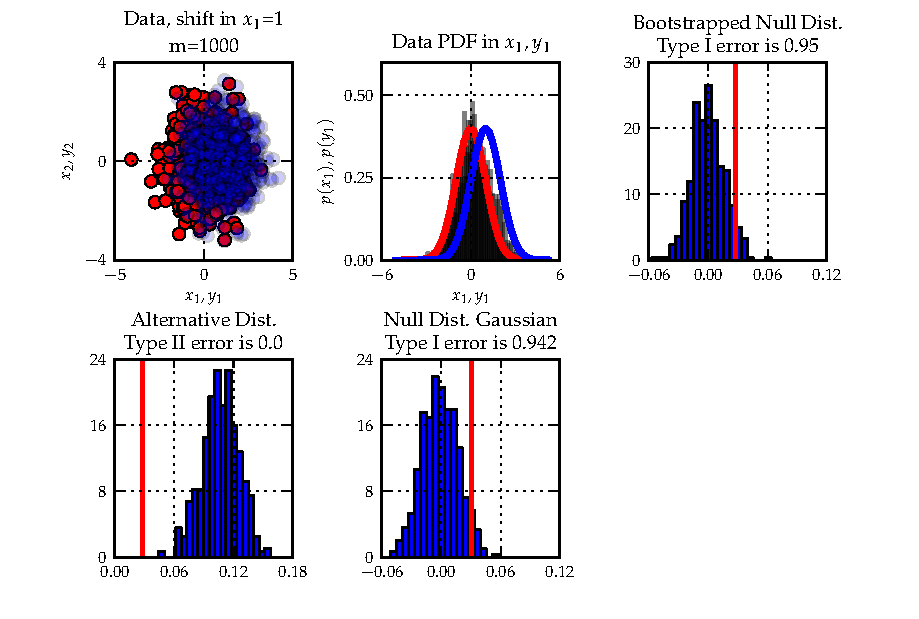
\includegraphics{fig/statistical_testing/linear_time_mmd}
		\caption{Screenshot of graphical python example for linear time MMD.}
		\label{fig:statistical_testing-linear_time_mmd}
\end{figure}

\begin{figure}\centering
		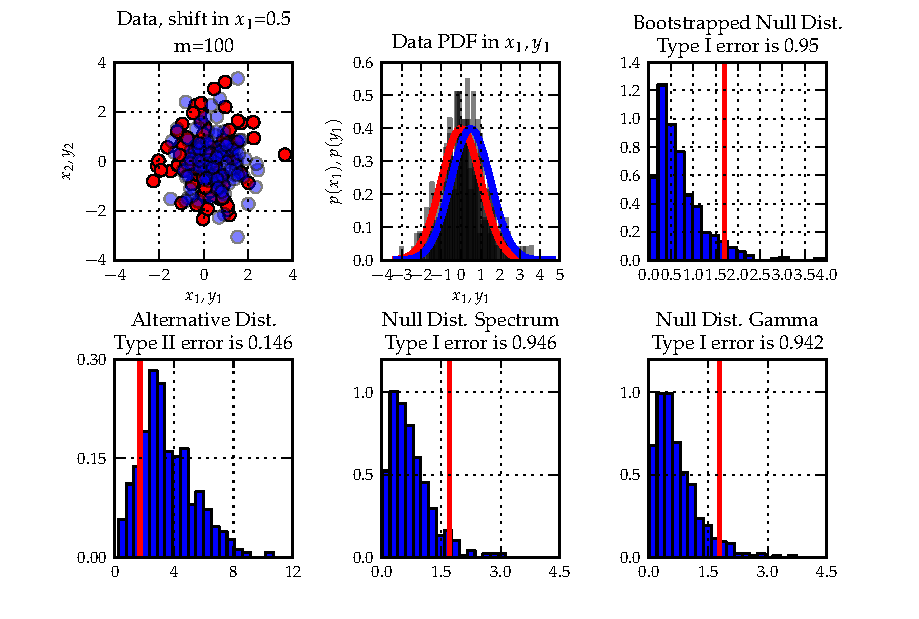
\includegraphics{fig/statistical_testing/quadratic_time_mmd}
		\caption{Screenshot of graphical python example for quadratic time MMD.}
		\label{fig:statistical_testing-quadratic_time_mmd}
\end{figure}
% Permission is granted to copy, distribute and/or modify this document
% under the terms of the GNU Free Documentation License, Version 1.3
% or any later version published by the Free Software Foundation;
% with no Invariant Sections, no Front-Cover Texts, and no Back-Cover Texts.
% A copy of the license is included in the section entitled "GNU
% Free Documentation License".
%
% Written (C) 2012 Heiko Strathmann

\section{Independence Testing with the HSIC Statistic}
\label{sec:hsic_test}

Independence testing tries to solve the following problem (taken from \citep{Gretton2008d}):
Let $\textbf{P}_{xy}$ be a Borel probability measure defined on a domain $\mathcal{X}\times\mathcal{Y}$, and let $\textbf{P}_x$ and $\textbf{P}_y$ be the respective marginal distributions on $\mathcal{X}$ and $\mathcal{Y}$. Given samples $Z=(X,Y)=\{(x_1, y_1), ..., (x_m, y_m)\}$ of size $m$ drawn independently and identically distributed according to $\textbf{P}_{xy}$, does $\textbf{P}_{xy}$ factorise as $\textbf{P}_{xy}=\textbf{P}_x \textbf{P}_y$? This corresponds to the question: Are $\textbf{P}_x$ and $\textbf{P}_y$ statistically independent? An independence test will distinguish between the hypothesises
\begin{align*}
H_0: \textbf{P}_{xy}=\textbf{P}_x \textbf{P}_y\\
H_1: \textbf{P}_{xy}\neq\textbf{P}_x \textbf{P}_y\\
\end{align*}

As for two-sample-testing, it is desirable to have a statistic that is zero if and only if $\textbf{P}_x$ and $\textbf{P}_y$ are independent. The so-called \emph{Hilbert Schmidt Independence Criterion} has this property. It is the squared Hilbert-Schmidt norm of the cross-covariance operator. We will now briefly describe where it comes from.

Let $\mathcal{F}$ be a RKHS with continuous feature mapping $\phi:\mathcal{X}\rightarrow\mathcal{F}$ and kernel $k:\mathcal{X}\times\mathcal{X}\rightarrow\mathbb{R}$ such that $\langle \phi(x)\phi(x')\rangle_\mathcal{F}=k(x,x')$; let $\mathcal{G}$ be another RKHS with continuous feature mapping $\psi:\mathcal{X}\rightarrow\mathcal{G}$ and kernel $l:\mathcal{Y}\times\mathcal{Y}\rightarrow\mathbb{R}$ such that $\langle \psi(y)\psi(y')\rangle_\mathcal{G}=k(y,y')$. The cross-covariance operator $C_{xy}:\mathcal{G}\rightarrow\mathcal{F}$ is defined such that for all $f\in\mathcal{F}$ and $g\in\mathcal{G}$
\begin{align*}
\langle f,C_{xy}g \rangle_\mathcal{F}=\textbf{E}_{xy}([f(x)-\textbf{E}_x(f(x))][g(y)-\textbf{E}_y (g(y))]
\end{align*}
The operator itself can be written as
\begin{align*}
C_{xy}=\textbf{E}_{xy}(\phi(x)-\mu_x) \otimes
 (\psi(y) - \mu_y)]
\end{align*}
where $\otimes$ is the tensor product. This is the generalisation of the cross-covariance matrix between random vectors in a RKHS. When $\mathcal{F}$ and $\mathcal{G}$ are \emph{universal}, then $||C_{xy}||$ is z is zero if and only if $H_0:\textbf{P}_{xy}=\textbf{P}_x \textbf{P}_y$ holds. Collecting everything gives the population expression for the HSIC. Let $x', y'$ be independent copies of the random variables $x,y$ respectively.
\begin{align}
\label{eqn:hsic_population}
\hsic[\textbf{P}_{xy},\mathcal{F},\mathcal{G}]=\textbf{E}_{xx'yy'}[k(x,x')l(y,y')] &+ \textbf{E}_{xx'}[k(x,x')]\textbf{E}_{yy'}[l(y,y')]\\
&-2\textbf{E}_{xy}[\textbf{E}_{x'}[k(x,x')]\textbf{E}_{y'}[l(y,y')]\notag
\end{align}

See \citep{Gretton2008d} for details. \shogun{} implements a biased estimator of the HSIC along with various methods to approximate its null distribution.

\subsection{Estimate of HSIC}
We now describe the method to estimate the HSIC that is implemented in \shogun{}, as described in \citep[Equation 4]{Gretton2008d}. All methods are implemented in \shogunclass{CHSIC}. The HSIC statistic has quadratic time and space costs, since it involves computing full kernel matrices and centring them.

A biased estimator for expression \ref{eqn:hsic_population} is given by
\begin{align*}
\hsic_b[(X,Y),\mathcal{F},\mathcal{G}]=\frac{1}{m^2}\trace(\textbf{KHLH})
\end{align*}
where $\textbf{K}, \textbf{L}$ are the full kernel matrices of kernels $k, l$ respectively and $\textbf{H}=\textbf{I}-\frac{1}{m}\textbf{1}\textbf{1}^T$ is a centring matrix with $\textbf{1}$ being a $m\times m$ matrix of ones. In \shogun{}, this expression is not evaluated using matrix multiplication, but the centring is done by hand. Call \texttt{compute\_statistic} in order to compute the estimate. Note that the method returns $m\hsic_b[(X,Y),\mathcal{F},\mathcal{G}]$ since null distribution approximations work on $m$ times null distribution.

\subsubsection{Bootstrapping}
As for any independence test in \shogun{}, bootstrapping can be used to approximate the null-distribution with any type of statistic. This results in a consistent, but slow test. Note that for each sample, the HSIC estimate has to be re-computed. The number of samples to take is the only parameter. As a rule of thumb, use at least 250 samples.
See \texttt{bootstrap\_null} in \shogunclass{CTwoDistributionsTestStatistic}, \shogunclass{CKernelIndependenceTestStatistic}, and \shogunclass{CHSIC}. Note that since the full kernel matrices have to be stored anyway when computing the HSIC estimate, in \texttt{bootstrap\_null}, these are pre-computed automatically for the current bootstrapping instance.
Bootstrapping is the only consistent HSIC test that is implemented in \shogun{}.

\subsubsection{Gamma}
Another, fast but heuristic method for approximating the null distribution for the HSIC is by matching the first two moments of a gamma distribution to it \citep[Equation 9]{Gretton2008d}. This is not consistent but usually gives good results in practice. However, there are distributions which break the gamma test. Therefore, the type I error should always be monitored.

It uses
\begin{align}
\label{eqn:hsic_gamma}
m\hsic_b(Z) \sim \frac{x^{\alpha-1}\exp(-\frac{x}{\beta})}{\beta^\alpha \Gamma(\alpha)}
\end{align}
where
\begin{align*}
\alpha=\frac{(\textbf{E}(\hsic_b(Z)))^2}{\var(\hsic_b(Z))} \qquad \text{and} \qquad
 \beta=\frac{m \var(\hsic_b(Z))}{(\textbf{E}(\hsic_b(Z)))^2}
\end{align*}

Then, any threshold and p-value can be computed using the gamma distribution in expression \ref{eqn:hsic_gamma}. Computational costs are in $\mathcal{O}(m^2)$, similar for space.

To use that method for testing, use \texttt{set\_null\_approximation\_method(HSIC\_GAMMA)}, to be found in \shogunclass{CHSIC}.

\subsubsection{Kernel Selection}
See section \ref{sec:statistical_tests-mmd-kernel_selection}. The same principle may be applied for HSIC-based tests. Note that since there is a kernel for each distribution, two kernel parameters have to be selected. Using the described median heuristic also leads to good results in some cases, as mentioned in \citep{Gretton2008d}.

\subsubsection{Example}
There is a graphical python example which plots example data, alternative and null-distributions. See figure \ref{fig:statistical_testing-hsic}.

\begin{figure}\centering
		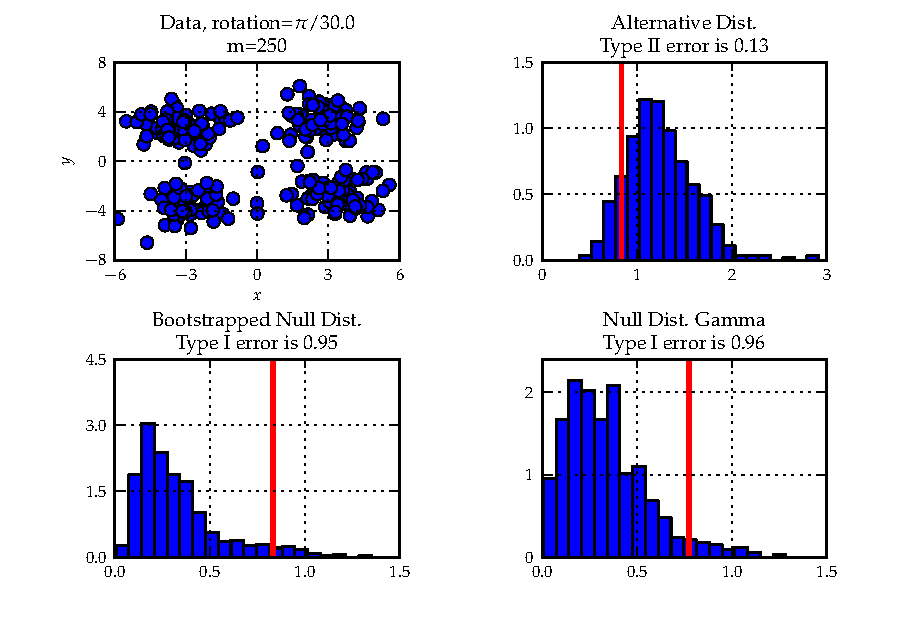
\includegraphics{fig/statistical_testing/hsic}
		\caption{Screenshot of graphical python example for HSIC.}
		\label{fig:statistical_testing-hsic}
\end{figure}
